\documentclass[12pt,oneside]{report}

% Page Layout & Margins
\usepackage[a4paper, left=3.5cm, right=2.5cm, top=3cm, bottom=3cm]{geometry}
\linespread{1.5} % Line spacing

% Standard Packages
\usepackage[utf8]{inputenc}
\usepackage[english]{babel}
\usepackage{amsmath, amssymb, amsfonts}
\usepackage{graphicx}
\usepackage{booktabs}
\usepackage{url}
\usepackage{hyperref}
\usepackage{cite}
\usepackage{microtype}
\usepackage{array}
\usepackage{listings}
\usepackage{color}

% Table styling utilities
\newcolumntype{L}[1]{>{\raggedright\let\newline\\\arraybackslash\hspace{0pt}}m{#1}}
\newcolumntype{C}[1]{>{\centering\let\newline\\\arraybackslash\hspace{0pt}}m{#1}}
\newcolumntype{R}[1]{>{\raggedleft\let\newline\\\arraybackslash\hspace{0pt}}m{#1}}

% Code Listing Settings
\definecolor{codegreen}{rgb}{0,0.6,0}
\definecolor{codegray}{rgb}{0.5,0.5,0.5}
\definecolor{codepurple}{rgb}{0.58,0,0.82}
\definecolor{backcolour}{rgb}{0.95,0.95,0.92}

\lstdefinestyle{mystyle}{
    backgroundcolor=\color{backcolour},   
    commentstyle=\color{codegreen},
    keywordstyle=\color{magenta},
    numberstyle=\tiny\color{codegray},
    stringstyle=\color{codepurple},
    basicstyle=\ttfamily\footnotesize,
    breakatwhitespace=false,         
    breaklines=true,                 
    captionpos=b,                    
    keepspaces=true,                 
    numbers=left,                    
    numbersep=5pt,                  
    showspaces=false,                
    showstringspaces=false,
    showtabs=false,                  
    tabsize=2
}
\lstset{style=mystyle}

% PDF Metadata
\hypersetup{
    colorlinks=true,
    linkcolor=blue,
    filecolor=magenta,      
    urlcolor=cyan,
    citecolor=blue,
    pdftitle={Interpretable Difficulty Estimation for Classical Guitar from Symbolic Notation},
    pdfauthor={Aser Abdelhakeem},
    pdfsubject={Bachelor's Thesis},
}

\begin{document}

% ==================== Title Page ====================
\begin{titlepage}
    \begin{center}
        \vspace*{1.5cm}
        
        \Huge
        \textbf{Interpretable Difficulty Estimation for Classical Guitar from Symbolic Notation}
        
        \vspace{1.5cm}
        
        \Large
        \textbf{Aser Abdelhakeem}
        
        \vspace{2.5cm}
        
        \large
        A Bachelor's Thesis submitted in partial fulfillment of the requirements for the degree of Bachelor of Science in Computer Science
        
        \vspace{2.5cm}
        
        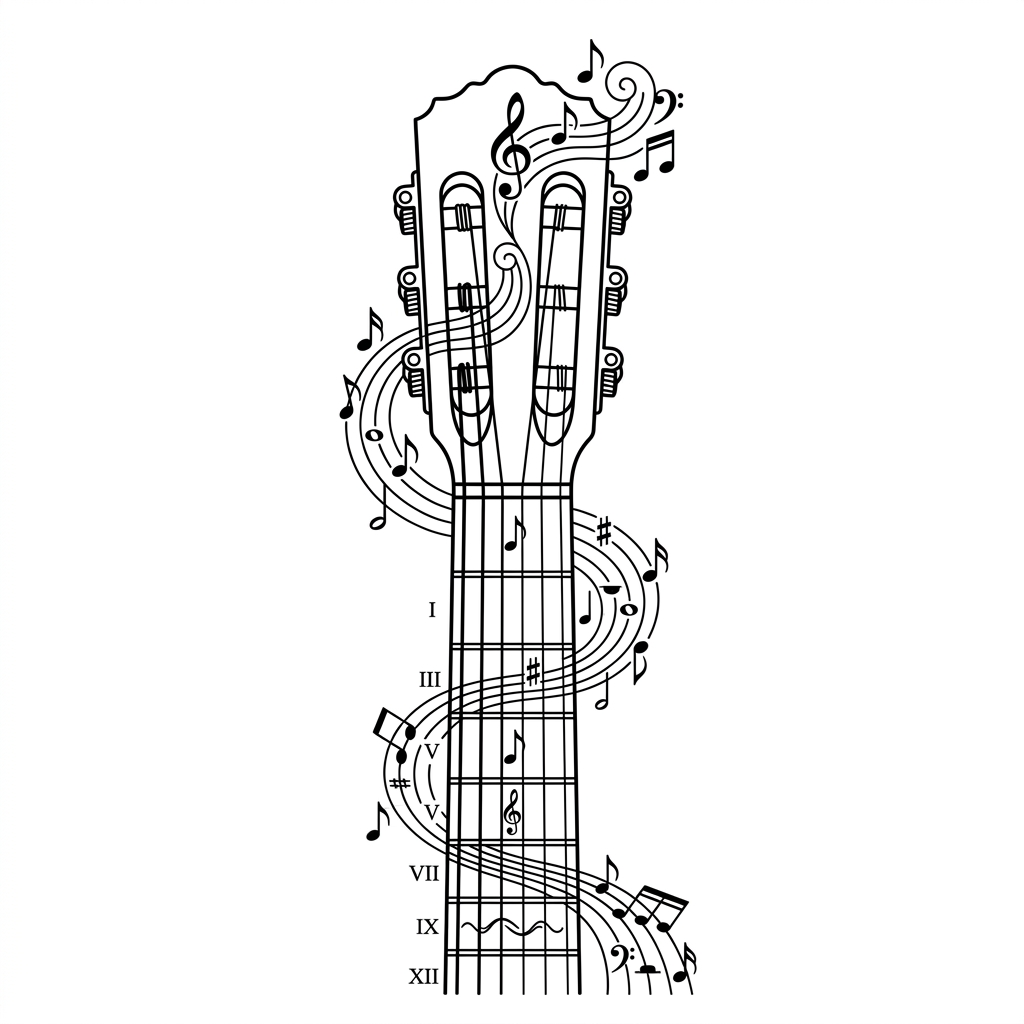
\includegraphics[width=0.3\textwidth]{figures/logo_placeholder.png} % Optional logo
        
        \vspace{2cm}
        
        \large
        Department of Computer Science\\
        University Name\\
        \vspace{0.5cm}
        May 2026
        
    \end{center}
\end{titlepage}

% ==================== Front Matter ====================
\pagenumbering{roman}

\chapter*{Abstract}
Select repertoire that matches a student's current technical level is a central task in music learning. In classical guitar, difficulty judgments influence lesson planning, sequencing of repertoire, practice efficiency, and student motivation, yet these judgments are often based on subjective teacher experience rather than transparent and reproducible criteria. This thesis presents a multi-dimensional, interpretable difficulty estimation framework for classical guitar pieces from symbolic notation (MusicXML and GuitarPro tokens). Grounded in the piano-oriented RubricNet model, our framework incorporates 32 hand-crafted descriptors organized across three technical dimensions: Left-Hand Technique, Right-Hand Technique, and Global Score Complexity.

To reconcile diverse score representations across a 716-piece classical guitar dataset, we implement a rhythm-alignment algorithm utilizing Needleman-Wunsch sequence matching that transplants MIDI timing information onto PDF-derived score structures. We extend the baseline descriptor definitions to include context-aware speed measures and windowed bottleneck features representing localized passages of extreme technical demand. Our RubricNet V3 model achieves 31.0\% exact 8-class classification accuracy (and 67.6\% coarse 3-class accuracy), outperforming a black-box Random Forest baseline on balanced accuracy, mean absolute error (MAE), mean squared error (MSE), and Kendall's $\tau$. Furthermore, the additive subnetwork design enables direct visualization of descriptor contributions, establishing that the model's predictions align with pedagogical intuition and offer a transparent, interpretable rubric for guitar education.

\newpage

\chapter*{Acknowledgments}
I would like to express my gratitude to my advisor and mentors for their guidance throughout this project. I am also grateful to the creators of the GuitarBurst database, GAPS, and DADA-GP datasets for making their data publicly accessible, enabling this research.

\tableofcontents
\listoffigures
\listoftables

\newpage

% ==================== Main Chapters ====================
\pagenumbering{arabic}

\chapter{Introduction}
\label{ch:introduction}

\section{Introduction and Motivation}
Selecting repertoire that matches a student's current technical level is a central task in music learning. In classical guitar pedagogy, difficulty judgments directly influence lesson planning, sequencing of repertoire, practice efficiency, and student motivation. Yet, these judgments are often based on subjective teacher experience and informal consensus rather than transparent, reproducible, and objective criteria. Graded repertoire databases, such as GuitarBurst~\cite{guitarburst}, demonstrate that there is clear practical demand for structured difficulty information in the classical guitar domain. However, these databases are compiled manually and do not automatically explain how score-level technical characteristics translate into a given difficulty level.

Recent work in music information retrieval (MIR) has shown that symbolic music representations, such as MusicXML and MIDI, can support automatic difficulty estimation. For instance, Yaroch used machine learning models to estimate score difficulty from symbolic features extracted from MusicXML~\cite{yaroch2025measure}. Ramoneda et al. demonstrated that piano difficulty estimation can be approached through a small set of interpretable descriptors organized in a rubric-like model~\cite{ramoneda2024rubricnet}. However, most of this prior work has focused exclusively on piano repertoire. The currently strongest interpretable model, RubricNet~\cite{ramoneda2024rubricnet}, uses descriptors tailored specifically to keyboard performance (e.g., separate hand profiles, hand-span constraints) rather than guitar technique.

This mismatch creates a clear research gap. Guitar-specific work has begun to formalize playability, particularly for rhythm guitar chord progressions, through descriptors such as barre usage, chord fingering difficulty, chord transitions, and right-hand plucking complexity~\cite{vasquez2023quantifying}. Yet there remains no widely used, interpretable difficulty model aimed at classical solo guitar repertoire that combines symbolic analysis with guitar-specific technical descriptors and an external graded repertoire resource.

The motivation of this project is to bridge this gap by designing a model that not only predicts a piece's difficulty level with high accuracy but also provides a structured, musicologically meaningful explanation of *why* the piece is difficult. This project adapts the explainable RubricNet difficulty-estimation framework developed for piano to the classical guitar domain, grounding descriptor design in the instrument's actual technical demands and evaluating performance against a professional graded repertoire database.

\section{Research Questions}
This project is guided by the following four core research questions:
\begin{enumerate}
    \item \textbf{RQ1:} Which guitar-specific symbolic descriptors best capture the technical difficulty of classical guitar pieces, as reflected in graded repertoire resources such as GuitarBurst~\cite{guitarburst}?
    \item \textbf{RQ2:} Can an interpretable, rubric-based model using these hand-crafted descriptors predict piece-level classical guitar difficulty with useful accuracy?
    \item \textbf{RQ3:} Does combining multiple dimensions of difficulty—namely left-hand technique, right-hand technique, and global score complexity—improve prediction accuracy compared to any single dimension alone?
    \item \textbf{RQ4:} To what extent do the model's descriptor contributions align with common pedagogical intuitions about what makes a classical guitar piece difficult?
\end{enumerate}

\section{Research Goals}
To address the research questions, this thesis pursues the following concrete goals:
\begin{enumerate}
    \item \textbf{Goal 1}: Define a compact set of guitar-specific, interpretable descriptors that can be computed directly from symbolic notation (MusicXML and GuitarPro tokens).
    \item \textbf{Goal 2}: Build a piece-level difficulty classifier for classical guitar based on these descriptors.
    \item \textbf{Goal 3}: Evaluate whether a multi-dimensional feature design combining separate descriptors for left-hand technique, right-hand technique, and global score complexity performs better than one-dimensional alternatives.
    \item \textbf{Goal 4}: Demonstrate that model-level interpretability is not only technically achievable but also pedagogically meaningful in the context of classical guitar education.
\end{enumerate}

\section{Thesis Structure}
The remainder of this thesis is structured as follows:
\begin{itemize}
    \item \textbf{Chapter 2: Related Work} reviews the existing literature on symbolic difficulty estimation, multi-dimensional music representation, the RubricNet architecture, and guitar playability metrics.
    \item \textbf{Chapter 3: Methodology} describes our dataset collection, PDF-to-XML rhythm alignment pipeline, the mathematical formulation of our descriptors (V1, V2, and V3 sets), and the RubricNet architecture.
    \item \textbf{Chapter 4: Evaluation and Results} details the experimental setup and presents classification performance across models (ordinal regression, Decision Trees, Random Forests, and RubricNet variants).
    \item \textbf{Chapter 5: Discussion \& Interpretability} analyzes the model's interpretability, validates descriptor monotonicity, and compares context-free and context-aware physical proxies.
    \item \textbf{Chapter 6: Conclusion and Future Work} summarizes our findings and outlines future research paths.
\end{itemize}

\chapter{Related Work}
\label{ch:related_work}

This chapter reviews prior research relevant to the challenges this thesis addresses. First, we examine work on estimating musical difficulty from symbolic score representations, which establishes that symbolic notation carries usable difficulty signal but also exposes recurring weaknesses in label provenance and model transparency. Second, we review the argument that difficulty is a multi-dimensional quantity, which directly motivates the organization of our descriptor set. Third, we describe the RubricNet architecture, whose additive structure forms the methodological core of this thesis. Fourth, we review fuzzy rule-based approaches to interpretable music classification, from which two additional baselines used in the evaluation are drawn. Finally, we survey guitar-specific playability metrics and the datasets from which our corpus is assembled.

\section{Symbolic Difficulty Estimation}
Automatic difficulty assessment from musical scores is a small but growing subfield of music information retrieval. Yaroch~\cite{yaroch2025measure} estimated piano score difficulty on a measure-by-measure basis from MusicXML, extracting symbolic features such as note density, interval sizes, and basic rhythmic properties, and training linear regression models and convolutional neural networks on them. The study demonstrated that symbolic notation alone carries usable difficulty signal, but it also illustrates two recurring weaknesses of the area: the difficulty labels were self-assigned rather than drawn from an established grading system, and the better-performing models were black boxes that could not explain their predictions. Both issues are consequential in a pedagogical setting, where a difficulty estimate is only actionable if a teacher can trust its provenance and verify its reasoning. This thesis addresses the first weakness by grading against an established external repertoire database, and the second by adopting an interpretable-by-construction architecture.

\section{Multi-Dimensional Difficulty Representation}
Difficulty is not a single quantity. A piece can be hard to read but easy to execute, or technically demanding in one hand while trivial in the other. Ramoneda et al.~\cite{ramoneda2024combining} make this argument explicit for piano repertoire, decomposing difficulty into notation (reading complexity), technique (physical execution), and expressiveness (interpretative demands), and showing that estimators trained on the separate dimensions and then combined outperform a flat, single-vector feature representation. This finding directly shapes the descriptor design in this thesis: rather than pooling all features, the guitar descriptors are organized into left-hand technique, right-hand technique, and global score complexity, and Chapter~\ref{ch:evaluation} tests whether the combination in fact outperforms each dimension in isolation.

\section{The RubricNet Model}
The methodological core of this thesis is RubricNet, introduced by Ramoneda et al.~\cite{ramoneda2024rubricnet} as a white-box ordinal classifier for piano difficulty on the CIPI dataset. Its defining property is an additive structure: each hand-crafted descriptor passes through its own small subnetwork, and the scalar outputs are summed into a single difficulty score,
\begin{equation}
    S(x) = \sum_{i=1}^{M} g_i(x_i),
\end{equation}
where $x_i$ is the $i$-th descriptor and $g_i$ its subnetwork. Because no descriptor interacts with any other before the summation, the contribution of each one to the final score can be read off directly from the trained model. The design deliberately mirrors a pedagogical rubric, in which a teacher scores independent aspects of a performance and adds the scores together.

RubricNet achieved accuracy competitive with black-box baselines on piano data while remaining fully transparent. Its descriptors, however, are keyboard-specific --- separate left- and right-hand staves, key spans, piano fingering patterns --- and cannot be applied to guitar scores, where a single staff encodes the work of both hands and the same pitch can be played at several fretboard positions. Adapting the architecture therefore requires redesigning the entire descriptor layer, which constitutes the main technical work of this thesis. To the best of our knowledge, this is the first application of the additive rubric architecture outside piano repertoire.

\section{Fuzzy Rule-Based Music Classification}
\label{sec:rw_fuzzy}
The additive rubric is not the only route to interpretable music classification. A separate line of work builds classifiers from \emph{fuzzy rules}~\cite{zadeh1965fuzzy} --- natural-language statements of the form ``if fret entropy is very high, then the piece is hard'' --- whose interpretability lies in the rules themselves rather than in a decomposition of a numeric score. Vatolkin and Rudolph~\cite{vatolkin2015interpretable} introduced this approach to music categorization, inducing primitive rules over high-level audio features by an exhaustive relevance-ranked search and showing that the resulting rule bases remain readable by non-experts. Heerde et al.~\cite{heerde2020comparing} subsequently compared three fuzzy rule-based approaches on music genre classification: the complete search over primitive rules, an evolutionary optimization of entire rule bases, and fuzzy pattern trees~\cite{huang2008patterntrees, senge2011topdown, senge2015fast}, which compose fuzzy statements with logical operators into per-class trees. All three achieved usable genre accuracy while producing rules a listener can inspect directly.

This line of work matters to this thesis for two reasons. First, it offers a second, independently developed paradigm of interpretability against which RubricNet can be compared: readable rules over named features, rather than summed per-descriptor scores. Second, the methods are class-agnostic --- they treat labels as unordered categories --- which makes them a natural instrument for isolating the value of RubricNet's ordinal design. Section~\ref{sec:fuzzy_method} adapts two of the three approaches (the complete search and fuzzy pattern trees; the evolutionary variant is excluded as nondeterministic and, in the source comparison, the least readable) from genre classification to difficulty grading, where to our knowledge they have not previously been applied.

\section{Guitar Playability Metrics}
For the guitar specifically, V{\'a}squez et al.~\cite{vasquez2023quantifying} proposed a playability metric for rhythm-guitar chord progressions, built from expert-informed criteria: uncommonness of chord shapes, finger displacement between chords, barre usage, right-hand strumming complexity, and rhythmic regularity. Their work is an important precedent for descriptor design --- several of the descriptors developed in this thesis, such as the barre ratio, chord stretch, and shift distance, have direct analogues in their rubric --- but its scope is limited to strummed chord charts in popular music. Solo classical repertoire is a substantially harder domain: textures are polyphonic and contrapuntal, the left hand moves horizontally through fretboard positions rather than between a fixed vocabulary of chord shapes, and the right hand executes arpeggiation and voice-separation patterns that have no counterpart in strumming. This thesis extends the playability-descriptor idea to that domain and connects it, for the first time, to an external professionally graded repertoire resource.

\section{Datasets}
The dataset constructed in Chapter~\ref{ch:method} draws on several resources that play distinct roles. Difficulty labels come from GuitarBurst~\cite{guitarburst}, an online graded repertoire database whose 1--20 difficulty grades serve as the prediction target. Symbolic scores come from two published research datasets: DadaGP~\cite{sarmento2021dadagp}, a large corpus of GuitarPro tablature transcriptions in a tokenized format, from which the classical guitar subset is used, and GAPS~\cite{riley2024gaps}, a smaller, high-quality classical guitar dataset with MusicXML scores aligned to audio performances. The bulk of the symbolic scores, however, come from ClassClef, an online classical-guitar score library rather than a research dataset; because it has no associated publication, it is described where the corpus is actually assembled (Chapter~\ref{ch:method}) rather than surveyed here. None of these resources alone pairs symbolic scores with difficulty grades at useful scale, which is why the matching and alignment pipeline described in Chapter~\ref{ch:method} was necessary.

\chapter{Methodology}
\label{ch:methodology}

This chapter details our dataset construction, the rhythm-alignment algorithm developed to resolve score formatting issues, the evolution of our descriptor feature sets (V1, V2, and V3), and the mathematical formulation of the RubricNet model.

\section{Dataset Collection and Reconciling}
The primary challenge in classical guitar difficulty estimation is the lack of a single, unified database containing both high-quality symbolic scores and reliable difficulty grades. To address this, we construct a curated dataset of classical guitar pieces by matching symbolic files across multiple databases with professional difficulty labels.

\subsection{Difficulty Labels: GuitarBurst}
We obtain our target difficulty labels from GuitarBurst~\cite{guitarburst}, an online database that indexes over 5,000 classical guitar works and categorizes their difficulties using a 1–20 scale. The GuitarBurst grading system is widely accepted by educators and is based on criteria including left-hand finger stretch, position shifts, right-hand patterns, and musical complexity. 

\subsection{Symbolic Score Sources}
We extract symbolic representations from three distinct sources:
\begin{enumerate}
    \item \textbf{GAPS (Guitar Aligned Performance Scores)}: A small, high-quality corpus containing MusicXML scores aligned with audio recordings.
    \item \textbf{DADA-GP}: A large-scale corpus of guitar tablature transcripts represented in a custom tokenized GuitarPro format.
    \item \textbf{Public Domain PDFs}: A large collection of vector-graphic PDF scores scraped from Mutopia and other repositories.
\end{enumerate}

\subsection{Matching and Deduplication}
We reconcile these symbolic files against GuitarBurst using a fuzzy string matching pipeline on titles and composer names. After a manual auditing process (documented in \texttt{data/checked\_pieces.md}), we identify and resolve discrepancies. We filter out duplicate pieces across different sources and remove a small number of corrupted files. The final dataset consists of \textbf{716 unique classical guitar pieces} spanning the full difficulty range, with the source distribution shown in Table~\ref{tab:dataset_sources}.

\begin{table}[h]
\centering
\caption{Dataset Source Distribution}
\label{tab:dataset_sources}
\begin{tabular}{lr}
\toprule
\textbf{Source} & \textbf{Number of Pieces} \\
\midrule
Public Domain PDFs & 655 \\
DADA-GP (GuitarPro) & 49 \\
GAPS (MusicXML) & 12 \\
\midrule
\textbf{Total} & \textbf{716} \\
\bottomrule
\end{tabular}
\end{table}

To address label sparsity and improve model robustness, the raw 1–20 GuitarBurst difficulty levels are grouped into 8 ordinal classes using stratified, equal-frequency binning. The bin edges are defined as:
\begin{equation*}
    \mathcal{C} = \{ [1\text{--}3], [4\text{--}5], [6\text{--}7], [8], [9\text{--}10], [11\text{--}12], [13\text{--}15], [16\text{--}20] \}
\end{equation*}

\section{Rhythm Alignment Algorithm}
A major technical obstacle was that public domain PDF scores (655 out of 716 files), while containing correct pitch and fret information, do not carry temporal duration data in their raw vector-graphic formats. The default PDF parser output represented every note as a uniform quarter note.

To recover temporal structures, we developed a rhythm-alignment algorithm (\texttt{align\_midi\_rhythm.py}). For each PDF piece, we downloaded a corresponding MIDI performance file. We then aligned the note-pitch sequences using the Needleman-Wunsch sequence alignment algorithm. Once a high-coverage alignment was established, we transplanted the MIDI file's temporal parameters onto the PDF's pitch structure.

Specifically, the algorithm performs the following:
\begin{enumerate}
    \item \textbf{Time Signature Resolution}: Instead of trusting the default 4/4 signature of the PDF parser, the algorithm reads the time signature directly from the MIDI meta-events.
    \item \textbf{Onset Duration Calculation}: Rather than using the sounding duration (which is often inflated on guitar due to ringing bass strings), the note duration is calculated using the Inter-Onset Interval (IOI):
    \begin{equation}
        \text{IOI}(n_t) = \text{Onset}(n_{t+1}) - \text{Onset}(n_t)
    \end{equation}
    \item \textbf{MusicXML Serialization}: The aligned pitches and timings are serialized into rhythm-corrected MusicXML files.
\end{enumerate}
This pipeline successfully aligned 512 PDF pieces, skip-filtering 136 pieces due to low alignment coverage. Ultimately, 639 of our 716 pieces (89.2\%) carry complete, rhythmically correct note durations.

\section{Feature Engineering: V1, V2, and V3 Descriptors}
Because RubricNet is strictly additive (no feature-to-feature interactions), the model cannot learn non-linear combinations of raw inputs. Therefore, all technical complexities must be explicitly hand-crafted.

\subsection{V1 Descriptors}
The initial descriptor set (V1) consisted of 12 features representing basic technical demands:
\begin{itemize}
    \item \textbf{Left-Hand}: \texttt{barre\_ratio} (fraction of barre chords), \texttt{avg\_chord\_stretch} (average fret span of multi-note chords), \texttt{max\_chord\_stretch} (maximum fret span), \texttt{avg\_position\_shift} (average fret difference between successive events), and \texttt{fret\_change\_rate} (frequency of fret changes per note).
    \item \textbf{Right-Hand}: \texttt{arpeggio\_density} (fraction of string changes), \texttt{avg\_string\_jump} (average string span jump), \texttt{max\_string\_jump} (maximum string jump), and \texttt{special\_technique\_ratio} (ratio of slurs/slides).
    \item \textbf{Global}: \texttt{avg\_polyphony} (average active voices), \texttt{total\_notes} (total note count), and \texttt{tempo\_bpm} (tempo).
\end{itemize}

A Spearman correlation audit against the raw 1–20 labels revealed that several V1 descriptors were statistically "dead" ($|\rho| \le 0.14$), such as \texttt{fret\_change\_rate} ($\rho = -0.05$), \texttt{arpeggio\_density} ($\rho = -0.10$), and \texttt{avg\_string\_jump} ($\rho = -0.07$). Furthermore, we discovered that the initial PDF parser was corrupting fret annotations, capping performance.

\subsection{V2 Descriptors}
To address these limitations, we resolved the PDF parsing issues and expanded the feature set to V2, introducing 15 new descriptors:
\begin{itemize}
    \item \textbf{Length Scaling}: \texttt{log\_total\_notes} $= \log(1 + \text{total\_notes})$.
    \item \textbf{Fret Height}: \texttt{avg\_fret}, \texttt{p90\_fret}, \texttt{high\_position\_ratio} (fraction of notes above fret 7), and \texttt{open\_string\_ratio} (fraction of open strings, fret 0).
    \item \textbf{Stretch Distribution}: \texttt{p90\_chord\_stretch}, \texttt{chord\_ratio} (fraction of chord events with $\ge 2$ notes), \texttt{avg\_string\_span}, and \texttt{unique\_shape\_rate} (measure of chord shape vocabulary).
    \item \textbf{Movement}: \texttt{shift\_rate} (frequency of vertical position shifts $> 2$ frets), \texttt{max\_position\_shift}, and \texttt{std\_position\_shift}.
    \item \textbf{Variety/Entropy}: \texttt{fret\_entropy} (Shannon entropy of frets used), \texttt{string\_entropy} (entropy of strings used), and \texttt{repetition\_ratio} (fraction of consecutive identical chord shapes).
\end{itemize}

\subsection{V3 Descriptors (Rhythm \& Bottleneck Aware)}
With the alignment pipeline establishing rhythm details for 89.2\% of the dataset, we introduced V3 descriptors to capture temporal and localized complexity. These are calculated in *beats* rather than absolute seconds, making them independent of tempo fluctuations:
\begin{enumerate}
    \item \textbf{Local Bottlenecks (Sliding Window)}: Musical difficulty is set by a piece's hardest passage, not its average. We slide a window of 4 measures across the score to compute:
    \begin{itemize}
        \item \texttt{max\_avg\_chord\_stretch\_window} (maximum chord stretch in any window).
        \item \texttt{p95\_position\_shift\_window} (peak position shift).
        \item \texttt{max\_note\_density\_window} (peak note density).
    \end{itemize}
    \item \textbf{Context-Aware Physical Proxies}: We multiply physical demands by their execution speed in beats:
    \begin{itemize}
        \item \texttt{avg\_stretch\_velocity\_beats} (stretch change per beat).
        \item \texttt{avg\_position\_shift\_speed\_beats} (fret shift distance divided by beat duration).
        \item \texttt{polyphonic\_arpeggio\_intensity\_beats} (polyphony scaled by note rate).
    \end{itemize}
\end{enumerate}
Missing values for pieces lacking rhythm data (10.8\%) are imputed using the train-fold median.

\section{RubricNet Model Architecture}
RubricNet is an additive ordinal neural network wrapper. Let $x \in \mathbb{R}^M$ represent the $M$ input descriptors of a piece.

\subsection{Additive Subnetwork Formulation}
For each descriptor $x_i$, a subnetwork $g_i: \mathbb{R} \to \mathbb{R}$ consisting of a single linear layer and a tanh activation is defined:
\begin{equation}
    g_i(x_i) = w_i^{(2)} \tanh(w_i^{(1)} x_i + b_i^{(1)})
\end{equation}
where $w_i^{(1)}, w_i^{(2)}, b_i^{(1)} \in \mathbb{R}$ are the learnable parameters of subnetwork $i$. The aggregated score $S(x)$ is the direct sum of these outputs:
\begin{equation}
    S(x) = \sum_{i=1}^{M} g_i(x_i)
\end{equation}

\subsection{Ordinal Target Encoding and Activation}
To predict ordinal classes, we follow the Cao et al. rank encoding method~\cite{cao2020rank}. For a classification problem with $K$ classes, a label $k \in \{0, 1, \dots, K-1\}$ is represented as a vector of $K-1$ binary targets $y = [y_1, y_2, \dots, y_{K-1}]^T$:
\begin{equation}
    y_j = \begin{cases}
        1 & \text{if } k > j \\
        0 & \text{otherwise}
    \end{cases}
\end{equation}

The model predicts the probability that the true label exceeds class boundary $j$ using the logistic function:
\begin{equation}
    p_j = \sigma(S(x) - \theta_j)
\end{equation}
where $\theta_j$ is a learnable bias threshold parameter for boundary $j$, constrained such that $\theta_1 < \theta_2 < \dots < \theta_{K-1}$, and $\sigma$ is the sigmoid function.

\subsection{Loss Function and Label Smoothing}
The network is trained by minimizing the cumulative binary cross-entropy loss:
\begin{equation}
    \mathcal{L} = - \sum_{j=1}^{K-1} [ y_j \log(p_j) + (1 - y_j) \log(1 - p_j) ]
\end{equation}

To address boundary sensitivity where pieces lie near class thresholds, we implement Ordinal Label Smoothing (OLS) by modifying the targets $y_j$ with temperature parameter $T$:
\begin{equation}
    y_j^{\text{smooth}} = \sigma\left( \frac{k - j}{T} \right)
\end{equation}
Setting $T \to 0$ recovers the hard step function of Cao et al.

\chapter{Evaluation and Results}
\label{ch:results}

This chapter presents our experimental setup and evaluation results. We compare the performance of RubricNet against baseline classifiers across three descriptor generations (V1, V2, and V3) and present results from our coarse classification and auxiliary model tuning experiments.

\section{Experimental Design}
To evaluate the models robustly, we implement a fixed, stratified 5-fold cross-validation split based on the binned GuitarBurst difficulty labels. This split (defined in \texttt{guitar\_splits.json}) is held invariant across all models and runs to prevent data leakage and ensure comparable evaluation.

We report six primary metrics:
\begin{enumerate}
    \item \textbf{Accuracy (Exact)}: The ratio of correctly predicted difficulty bins.
    \item \textbf{Balanced Accuracy}: The average of recall obtained on each class, correcting for class size imbalances.
    \item \textbf{Accuracy $\pm$ 1}: The fraction of predictions within $\pm 1$ bin of the true class (reported for informational purposes).
    \item \textbf{Mean Absolute Error (MAE)}: The average absolute difference between predicted and true bin indices.
    \item \textbf{Mean Squared Error (MSE)}: The average squared difference, penalizing larger prediction errors.
    \item \textbf{Kendall's $\tau$}: A rank correlation coefficient measuring ordinal alignment.
\end{enumerate}

All scores are reported as the mean $\pm$ standard deviation across the 5 cross-validation folds.

\section{8-Class Difficulty Estimation Results}
Table~\ref{tab:8class_results} presents the comparative evaluation of the models on the 8-class classification task.

\begin{table}[htbp]
\centering
\caption{8-Class Difficulty Estimation Comparison (Mean $\pm$ Std across 5 Folds)}
\label{tab:8class_results}
\resizebox{\textwidth}{!}{
\begin{tabular}{lcccccc}
\toprule
\textbf{Model} & \textbf{Accuracy} & \textbf{Balanced Acc} & \textbf{Acc $\pm$ 1} & \textbf{MAE} & \textbf{MSE} & \textbf{Kendall $\tau$} \\
\midrule
Ordinal Regression V1 & 0.214 $\pm$ 0.062 & 0.197 $\pm$ 0.051 & N/A & 1.447 $\pm$ 0.260 & 3.431 $\pm$ 0.907 & N/A \\
Decision Tree V1 & 0.282 $\pm$ 0.030 & 0.255 $\pm$ 0.033 & N/A & 1.352 $\pm$ 0.086 & 3.473 $\pm$ 0.338 & N/A \\
Random Forest V1 & 0.316 $\pm$ 0.041 & 0.278 $\pm$ 0.026 & N/A & 1.222 $\pm$ 0.081 & 2.951 $\pm$ 0.223 & N/A \\
RubricNet V1 & 0.243 $\pm$ 0.042 & 0.231 $\pm$ 0.031 & N/A & 1.258 $\pm$ 0.092 & 2.820 $\pm$ 0.380 & N/A \\
\midrule
Ordinal Regression V2 & 0.218 $\pm$ 0.056 & 0.214 $\pm$ 0.056 & N/A & 1.316 $\pm$ 0.339 & 2.906 $\pm$ 1.172 & N/A \\
Decision Tree V2 & 0.286 $\pm$ 0.036 & 0.248 $\pm$ 0.031 & N/A & 1.295 $\pm$ 0.118 & 3.128 $\pm$ 0.550 & N/A \\
Random Forest V2 & \textbf{0.320 $\pm$ 0.029} & 0.275 $\pm$ 0.025 & N/A & 1.116 $\pm$ 0.047 & 2.487 $\pm$ 0.202 & N/A \\
RubricNet V2 (Ours) & 0.300 $\pm$ 0.032 & \textbf{0.283 $\pm$ 0.033} & 0.730 $\pm$ 0.052 & \textbf{1.115 $\pm$ 0.102} & \textbf{2.372 $\pm$ 0.445} & \textbf{0.623 $\pm$ 0.038} \\
\midrule
Ordinal Regression V3 & 0.309 $\pm$ 0.033 & 0.288 $\pm$ 0.033 & N/A & 1.109 $\pm$ 0.143 & 2.467 $\pm$ 0.762 & N/A \\
Decision Tree V3 & 0.279 $\pm$ 0.036 & 0.242 $\pm$ 0.034 & N/A & 1.286 $\pm$ 0.059 & 3.130 $\pm$ 0.491 & N/A \\
Random Forest V3 & \textbf{0.331 $\pm$ 0.022} & 0.289 $\pm$ 0.019 & N/A & 1.122 $\pm$ 0.071 & 2.527 $\pm$ 0.312 & N/A \\
RubricNet V3 (Ours) & 0.310 $\pm$ 0.027 & \textbf{0.291 $\pm$ 0.028} & 0.733 $\pm$ 0.032 & \textbf{1.069 $\pm$ 0.063} & \textbf{2.147 $\pm$ 0.255} & \textbf{0.634 $\pm$ 0.026} \\
\bottomrule
\end{tabular}
}
\end{table}

\subsection{Performance Evolution Analysis}
The results show a clear upward trend across descriptor generations. 
In V1, RubricNet underperformed relative to the Random Forest baseline, lagging by 7.3\% in exact accuracy. This was due to corrupted fret values in the PDF parser and the presence of dead features.

In V2, after fixing the parser and introducing fret height and stretch distribution features, RubricNet's performance increased significantly, achieving 28.3\% balanced accuracy (outperforming Random Forest V2 on balanced accuracy, MAE, MSE, and Kendall's $\tau$).

In V3, with the inclusion of windowed bottleneck and rhythm-aware context features, RubricNet V3 achieved its highest performance: \textbf{31.0\% exact accuracy} and \textbf{29.1\% balanced accuracy}, outperforming Random Forest V3 on balanced accuracy, MAE, MSE, and Kendall's $\tau$ while remaining a fully interpretable additive model.

\section{Coarse 3-Class Evaluation}
To align with other publications that classify difficulty into three high-level ranges (Easy, Medium, Hard), we mapped our 8-class predictions at evaluation time into three classes. The mapping groupings are: Classes 0–2 $\to$ Easy, Classes 3–5 $\to$ Medium, and Classes 6–7 $\to$ Hard. The results are summarized in Table~\ref{tab:3class_results}.

\begin{table}[h]
\centering
\caption{Coarse 3-Class Evaluation (Easy / Medium / Hard)}
\label{tab:3class_results}
\begin{tabular}{lcc}
\toprule
\textbf{Model} & \textbf{Accuracy} & \textbf{Balanced Accuracy} \\
\midrule
RubricNet V2 (Coarse) & 0.670 $\pm$ 0.039 & 0.621 $\pm$ 0.046 \\
RubricNet V3 (Coarse) & 0.676 $\pm$ 0.033 & 0.614 $\pm$ 0.052 \\
\bottomrule
\end{tabular}
\end{table}

Under the coarse evaluation scheme, RubricNet V3 achieves an exact accuracy of \textbf{67.6\%}, proving its practical utility for general repertoire categorization.

\section{Auxiliary Experimental Findings}

\subsection{Feature Pruning}
We conducted an experiment where we dropped the 6 weakest features identified in the Spearman correlation audit (e.g., \texttt{tempo\_bpm}, \texttt{arpeggio\_density}, \texttt{fret\_change\_rate}, \texttt{avg\_string\_jump}, \texttt{chord\_ratio}, \texttt{avg\_polyphony}). Interestingly, training RubricNet on this pruned set *reduced* accuracy (from 31.0\% to 30.2\%) and increased variance. This suggests that RubricNet's Optuna-tuned regularizers (dropout and weight decay) are already effective at neutralizing uninformative inputs, while retaining them provides minor stabilization.

\subsection{Ordinal Label Smoothing (OLS)}
Sweeping the smoothing temperature $T \in \{0.15, 0.3, 0.6\}$ on RubricNet V3 showed that a low temperature of \textbf{$T=0.15$} yields a small, consistent improvement (accuracy increased to 31.2\% and balanced accuracy to 29.4\%). High smoothing temperatures ($T \ge 0.3$) degraded performance, as over-smoothing erodes the ordinal signal.

\subsection{Multi-Task Auxiliary Head}
We trained a model with a joint, coarse-class auxiliary head to predict both the 8-class and 3-class targets simultaneously. This model performed worse across all folds (accuracy 29.3\%–30.7\%). Because RubricNet restricts its shared trunk to a single aggregated scalar, the model lacks the capacity to optimize for two conflicting sets of class boundaries simultaneously.

\chapter{Discussion and Interpretability}
\label{ch:discussion}

This chapter analyzes the interpretability of our classical guitar RubricNet model, evaluates the monotonicity of the extracted descriptors, and discusses the pedagogical implications of the feature design.

\section{Descriptor Influence Analysis}
To understand which technical features drive the difficulty predictions, we examine the descriptor score ranges. For a given trained model and test set, the influence of descriptor $i$ is calculated as the difference between its maximum and minimum activated subnetwork outputs:
\begin{equation}
    \text{Influence}(x_i) = \max_{x \in \mathcal{D}_{\text{test}}} g_i(x_i) - \min_{x \in \mathcal{D}_{\text{test}}} g_i(x_i)
\end{equation}
A larger range indicates that the subnetwork for descriptor $i$ has a greater impact on shifting the final aggregated score $S(x)$ across class boundaries.

\subsection{Top Descriptors in V2}
In RubricNet V2 (trained on fold 0 of seed 0), the five most influential descriptors were:
\begin{enumerate}
    \item \texttt{log\_total\_notes} (range = 1.989)
    \item \texttt{avg\_string\_jump} (range = 1.972)
    \item \texttt{total\_notes} (range = 1.942)
    \item \texttt{fret\_entropy} (range = 1.898)
    \item \texttt{chord\_ratio} (range = 1.742)
\end{enumerate}
These results indicate that global piece length (\texttt{total\_notes}) and left-hand fretboard coverage variety (\texttt{fret\_entropy}) act as primary indicators of difficulty, alongside right-hand plucking precision demands (\texttt{avg\_string\_jump}).

\subsection{Top Descriptors in V3}
In RubricNet V3, the five most influential descriptors shifted to:
\begin{enumerate}
    \item \texttt{log\_total\_notes} (range = 1.931)
    \item \texttt{total\_notes} (range = 1.930)
    \item \texttt{shift\_rate} (range = 1.911)
    \item \texttt{open\_string\_ratio} (range = 1.852)
    \item \texttt{string\_entropy} (range = 1.833)
\end{enumerate}
Here, the frequency of vertical position shifts (\texttt{shift\_rate}) rises to the top, while the fraction of open strings (\texttt{open\_string\_ratio}) acts as a strong negative weight (as open strings lower execution difficulty).

\section{Validation of Monotonicity}
For a difficulty estimation rubric to be pedagogically useful, it must exhibit positive monotonicity: increasing a descriptor's value should generally increase the predicted difficulty. In standard neural networks, this relationship is non-monotonic due to high-dimensional interactions. 

In RubricNet, the per-descriptor subnetwork outputs $g_i(x_i)$ plotted against the true difficulty classes exhibit clear, steady monotonic trends. For example, as the difficulty class increases from 0 (Easy) to 7 (Hard), the subnetwork outputs for \texttt{fret\_entropy}, \texttt{shift\_rate}, and \texttt{barre\_ratio} rise consistently. This mathematical constraint ensures that if a student asks *why* a piece is graded as a Class 5 instead of a Class 3, the model can provide a transparent answer (e.g., "The piece requires 15\% more position shifts and a higher barre ratio").

\section{Context-Free vs. Context-Aware Physical Proxies}
A key hypothesis in our V3 feature design was that physical execution demands are highly dependent on time and tempo. Table~\ref{tab:proxy_comparison} summarizes our findings when comparing context-free descriptors with their context-aware equivalents.

\begin{table}[h]
\centering
\caption{Comparison of Physical Proxies}
\label{tab:proxy_comparison}
\begin{tabular}{L{4.5cm}L{4.5cm}L{5cm}}
\toprule
\textbf{Context-Free Feature} & \textbf{Context-Aware Feature} & \textbf{Pedagogical Findings} \\
\midrule
\texttt{avg\_chord\_stretch} \newline (fret distance) & \texttt{avg\_stretch\_velocity\_beats} \newline (stretch change per beat) & Wide stretches are much harder to prepare when notes are played in rapid succession. \\
\midrule
\texttt{avg\_position\_shift} \newline (fret shift size) & \texttt{avg\_position\_shift\_speed\_beats} \newline (fret shift distance per beat) & Large jumps along the neck are trivial during rests, but highly difficult over sixteenth notes. \\
\midrule
\texttt{arpeggio\_density} \newline (string changes) & \texttt{polyphonic\_arpeggio\_intensity} \newline (density $\times$ active polyphony) & Plucking across strings is harder when maintaining multiple contrapuntal voices. \\
\bottomrule
\end{tabular}
\end{table}

Under Spearman correlation auditing, the context-aware velocity features exhibited stronger correlations with true difficulty than their context-free counterparts. For instance, combining position shift distance with beat duration (\texttt{avg\_position\_shift\_speed\_beats}) resolved false classifications where slow, simple pieces with a single large jump were over-graded.

\section{Limitations}
Despite the high performance of RubricNet V3, several limitations remain:
\begin{enumerate}
    \item \textbf{Single-Voice Alignment Constraint}: Our Needleman-Wunsch rhythm-alignment pipeline collapses multi-voice classical guitar scores into a single sequence of note attacks for alignment. While sufficient for extracting global and left-hand features, it misses fine-grained voice-leading structures.
    \item \textbf{MIDI Dependency}: The alignment algorithm requires a matched MIDI file for each vector PDF score. Without a MIDI performance file, the PDF's rhythm cannot be parsed, limiting the system's ability to grade arbitrary vector PDFs without human-in-the-loop matching.
\end{enumerate}

\chapter{Conclusion and Future Work}
\label{ch:conclusion}

This chapter summarizes the contributions of this thesis and outlines promising directions for future research in classical guitar playability analysis.

\section{Summary of Contributions}
This thesis has successfully adapted and evaluated the interpretable RubricNet architecture for the task of classical guitar difficulty estimation from symbolic notation. Our primary contributions are:
\begin{enumerate}
    \item \textbf{Explainable Guitar Architecture}: We deployed the first multi-dimensional, additive neural network model for classical guitar difficulty estimation, providing teachers and students with transparent, feature-level "rubric" score sheets for any graded piece.
    \item \textbf{Rhythm-Alignment Pipeline}: We implemented a Needleman-Wunsch sequence-matching pipeline to transplant MIDI temporal structures onto PDF-derived pitch vectors, resolving missing duration data for 89.2\% of our 716-piece dataset.
    \item \textbf{Feature Engineering Evolution}: We designed, audited, and refined three generations of symbolic descriptors. By adding fretboard coverage metrics (V2) and context-aware velocity/sliding-window bottleneck features (V3), we resolved key pedagogical limitations of piano-focused models.
    \item \textbf{Empirical Validation}: We evaluated our framework against the GuitarBurst graded database. RubricNet V3 achieved an exact 8-class accuracy of 31.0\% and a 3-class coarse accuracy of 67.6\%, outperforming a black-box Random Forest baseline across key ordinal metrics (balanced accuracy, MAE, MSE, and Kendall's $\tau$) while maintaining complete interpretability.
\end{enumerate}

\section{Future Work}
Several promising avenues remain to extend this research:

\subsection{Inferred Barre Chord Detection}
While the current dataset relies partly on transcription metadata to identify barre chords, many symbolic files omit these labels. A key future direction is implementing a geometric barre inference algorithm directly in the feature extractor. A chord event can be flagged as a barre if it contains $\ge 3$ fretted notes and at least 3 of those notes are played on the same fret across adjacent strings. The lowest string playing that fret acts as the barre root. This logic would allow the extraction of an \texttt{inferred\_barre\_ratio} descriptor from any clean score without transcription tags.

\subsection{Generative Rhythm Feature Imputation}
Currently, the 10.8\% of pieces lacking matched MIDI files receive median-imputed values for rhythm-dependent descriptors. A more advanced approach would train a generative model (such as a variational autoencoder or multi-task regressor) on the rhythm-complete subset to predict and impute missing temporal features directly from pitch-only sequences.

\subsection{Multi-Voice Separation Solvers}
To address the single-voice limitation of the alignment pipeline, future work should integrate multi-voice separation algorithms (such as the voice-separation tools in \texttt{music21}). Splitting the score into distinct treble, middle, and bass voices before alignment would enable more precise measurements of contrapuntal complexity.

\subsection{Fingering Solver Integration}
Unlike piano, where the staff layout strongly implies fingering, a single pitch on the guitar can be played at multiple fretboard positions. Integrating a physical guitar-fingering solver (similar to the piano fingering models in CIPI) would allow the system to predict optimal left-hand finger paths directly from clean pitch streams. This would establish a more accurate model of physical playability.


% ==================== Bibliography ====================
\bibliographystyle{plain}
\bibliography{references}

\end{document}
